\chapter{Multiprocessadores Simétricos}

\section{Classificação de Arquiteturas}

A divisão das arquiteturas de Flynn possui quatro categorias, segundo o numero de instruções executadas e dados acessados em um instante. Esta divisão foi o primeiro passo na classificação de arquiteturas paralelas e distribuídas. É considerada imprecisa. A Figura \ref{figs:arch-procs} dá a visão geral de todas.

\begin{figure}
  \centering
  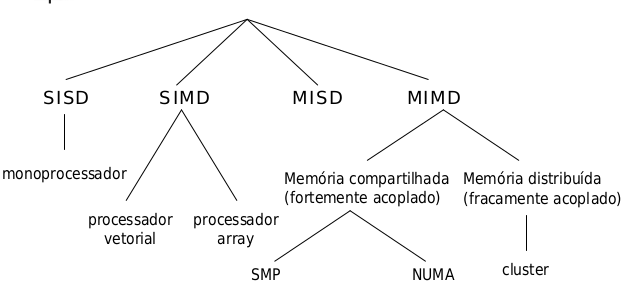
\includegraphics[width=0.9\textwidth]{archs-tree}
  \caption{Taxonomia das Arquiteturas, por Stallings}
  \label{fig:archs-tree}
\end{figure}

\subsubsection{Single Instruction, Single Data (SISD)}
Processadores pipeline e monoprocessadores se encaixam aqui. Possuem os seguintes componentes:

\begin{itemize}
  \item UC: unidade de controle
  \item UP: unidade de processamento, por exemplo a ULA
  \item MEM: memória
\end{itemize}

\subsubsection{Single Instruction, Multiple Data (SIMD)}
A extensão do SISD com multiplicação dos \textit{hardwares} de unidade de processamento e memória (processadores vetoriais). Uma única instrução é buscada e é posta em todos os processadores para execução em posições de memória diferentes. Esta arquitetura é muito usada em GPUs.

\subsubsection{Multiple Instruction, Single Data}
Busca de várias instruções para execução sob um mesmo dado em memória. Dessa forma a replicação está nas unidades de controle e processamento. Esta arquitetura não possui exemplo de caso real, por não fazer sentido.

\subsubsection{Multiple Instruction, Multiple Data (MIMD)}
É uma arquitetura equivalente a multiprocessadores (ou multicores). Além disso, redes de computadores também se encaixam neste exemplo, dado que as unidades representadas são abstratas. Possuem duas arquiteturas:

\begin{itemize}
  \item Fortemente acopladas: Todos os processadores tem acesso direto à memória, sendo ela \textbf{compartilhada}. Exemplo: multiprocessadores;

  \item Fracamente acopladas: cada processadore tem acesso direto apenas a sua memória. Para acesso à outras memórias, \textbf{deve} pedir para o processador detentor da memória alvo. Exemplos: multicomputadores.
\end{itemize}

\begin{figure*}
  \begin{subfigure}{.5\textwidth}
    \centering
    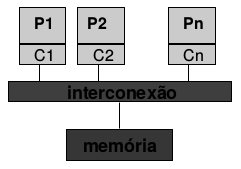
\includegraphics[width=\textwidth, height=4.5cm]{mimd-strong}
    \caption{Fortemente Acoplada}
  \end{subfigure}
  ~
  \begin{subfigure}{.5\textwidth}
    \centering
    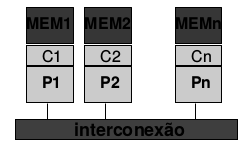
\includegraphics[width=\textwidth]{mimd-weak}
    \caption{Fracamente Acoplada}
  \end{subfigure}

  \caption{Tipos de Arquiteturas MIMD}
\end{figure*}

\begin{figure*}
  \begin{subfigure}{.5\textwidth}
    \centering
    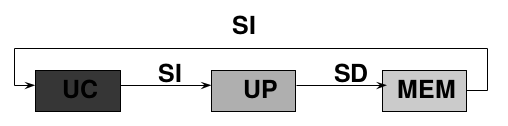
\includegraphics[width=\textwidth]{sisd}
    \caption{SISD}
  \end{subfigure}
  ~
  \begin{subfigure}{.5\textwidth}
    \centering
    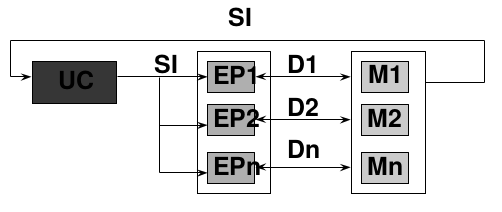
\includegraphics[width=\textwidth]{simd}
    \caption{SIMD}
  \end{subfigure}
  ~
  \begin{subfigure}{.5\textwidth}
    \centering
    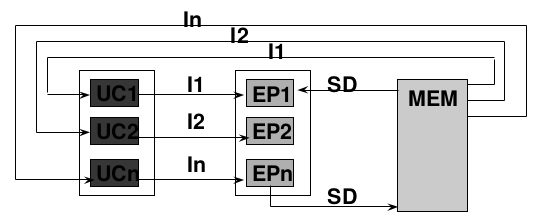
\includegraphics[width=\textwidth]{misd}
    \caption{MISD}
  \end{subfigure}
  ~
  \begin{subfigure}{.5\textwidth}
    \centering
    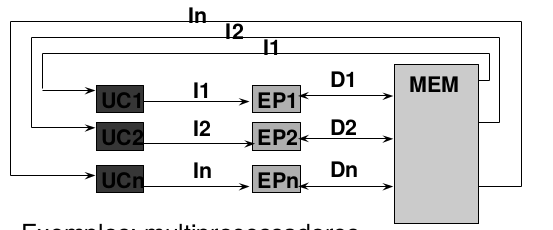
\includegraphics[width=\textwidth]{mimd}
    \caption{MIMD}
  \end{subfigure}

  \caption{Tipos de arquiteturas de processadores, segundo Flynn}
  \label{figs:arch-procs}
\end{figure*}




\section{Multiprocessadores Simétricos}

Inicialmente conhecidos como Uniform Memory Access Time (UMA). Possuem dois ou mais processadores com capacidade equivalentes, compartilhando memórias e sistema de I/O, interconectados por um barramento ou crossbar, sendo essa arquitetura \textbf{transparente ao usuário}.

Todos os processadores podem desempenhar as mesmas funções e o sistema é controlado por um sistema operacional integrado. É uma implementação relativamente simples, uma vez que apenas aumentamos o número de processados, mas mantendo mantendo a memória e barramento únicos.

\begin{figure}[ht]
  \centering
  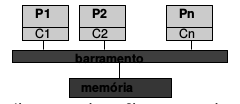
\includegraphics[width=0.6\textwidth]{smp}
  \label{fig:smp}
  \caption{Estrutura de um multiprocessador simétrico. A memória aqui não é necessariamente única}
\end{figure}

\begin{definicao}{\textit{Crossbar}}
  Vários barramentos de maneira que você consiga uma conexão direta com todos os barramentos, evitando conflito de acesso, porém sendo um \textit{hardware} mais caro. Ele é quadrátrico em relação ao número de elementos ($n^2$ conexões quando se tem $n$ elementos), permitindo a garantia de acesso em tempo uniforme.
\end{definicao}

Quando interconectados por barramentos, a arquitetura não é escalável, devido a problemas de contenção no acesso à memória. A cada processador adicionado, existe mais conflito no barramento. Com o crossbar, o problema é o custo do mesmo.

Assim, a introdução cache entre o processador e barramento aliviou um pouco o problema do acesso constante ao barramento, pois o acesso ficou local, gerenciado por algoritmos eficientes de coerência das caches.

Entretanto, mesmo com a introdução da cache, o número de processadores que podem ser conectados ao barramento não chega a 30, sendo geralmente 8. Para tentar resolver o problema de contenção em UMAs, foram propostas arquiteturas NUMA.




\section{Coerência de Cache}
As arquiteturas paralelas fortemente acopladas são afetadas por 3 grandes problemas.

\begin{itemize}
  \item \textbf{Contenção da memória:} ocorre pois cada módulo de memória só pode tratar uma requisição por vez. Logo as requisições para um mesmo módulo são enfileiradas.

  \item \textbf{Contenção de comunicação:} o tempo de latência para redes de interconexão é dado pelo tempo que uma requisição leva para atravessar a rede de interconexão. Isso é diferente de largura de banda, que é a quantidade de informação que pode ser transmitida por uma rede em um determinada tempo.

  \item Tempo de latência
\end{itemize}

As caches em multiprocessadores podem ser:
\begin{itemize}
  \item \textbf{Privadas:} cada processador tem sua cache;
  \item \textbf{Compartilhada:} só existe uma cache, compartilhada entre vários processadores
\end{itemize}

\begin{definicao}{Coerência de \textit{Cache}}
  Garantia que todas as caches possuem sempre o mesmo valor para todas as cópias dos dados, \textbf{quando observadas}.
\end{definicao}

Logo, queremos garantir que todas as cópias em cache retornem sempre o último valor escrito, ou seja, uma visão coerente e uniforme da memória para todos os processadores, independente do fato de existirem várias caches.

Um \textbf{protocolo de coerência de cache} consistem em:
\begin{itemize}
  \item Um conjunto de estados possíveis das caches locais;
  \item Um conjunto de estados possíveis da memória
  \item Transições de estados causadas por mensagem ou eventos locais.
\end{itemize}




Definimos então duas políticas parada garantir a coerência.

\textsc{Política 1:} \textbf{Write-invalidate}\\
Todas as cópias de um mesmo bloco são invalidadas antes que uma escrita/atualização seja feita em um processador.

Em caso de leitura, se a cópia existir localmente, a operação é feita também localmente. Caso não exista:
\begin{itemize}
  \item Se existir uma cópia em leitura, fazemos uma outra cópia do bloco

  \item Se existir uma cópia em escrita:
  \begin{itemize}
    \item Fazemos uma cópia do bloco e invalidamos a cópia em escrita; ou
    \item Fazemos uma cópia do bloco e tornamos a cópia em escrita um \textit{read-only}
  \end{itemize}
\end{itemize}

\textbf{Premissa:} quando é observada a escrita de um bloco compartilhado, \textbf{invalide} seu bloco.

\underline{Exemplo:} processador $P_1$ quer escrever na sua cache $C_1$ no bloco $b$. Ele avisa aos demais processadores sobre a escrita. Agora, cada processador $P_i$ analisa se ele possui uma cópia de $b$ e caso positivo, ele invalida a cópia. Ao fim, $P_1$ escreve o dado em sua cache. Se $P_i$ desejar obter o bloco invalidado, terá que buscar da memória.\\


\textsc{Política 2:} \textbf{Write-update}\\
As escritas são feitas de maneira atômica em todas cópias dos blocos. Ou seja, assim que uma escrita de um bloco em cache é percebida, a cache solicita o bloco da memória.

\textbf{Premissa:} quando é observada a escrita de um bloco compartilhado, \textbf{atualize} seu bloco.

\underline{Exemplo:} processador $P_1$ quer escrever na sua cache $C_1$ no bloco $b$. Ele avisa aos demais processadores sobre a escrita. Agora, cada processador $P_i$ analisa se ele possui uma cópia de $b$ e caso positivo, ele busca a cópia atualizada e a atualiza. Depois, $P_1$ escreve o dado em sua cache e libera o barramento. No fim, todas as caches estão com os dados atualizados.





\section{Snoopy Caches}
Em arquiteturas conectadas por um barramentos, broadcasts são feitos a cada operação de coerência e assim, as caches sempre estão "escutando" a rede para receber os comandos de coerência. Ao receber um comando, checam se possuem o bloco referênciado e, caso afirmativo, aplicam a operação de coerência. \textbf{Uma cache que implementa esse comportamento é uma snoopy cache}.

\begin{figure}
  \centering
  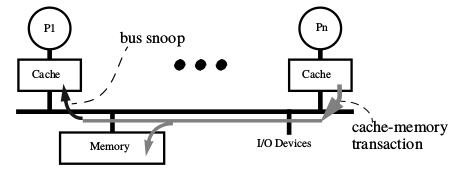
\includegraphics[width=0.8\textwidth]{snoopy-cache}
  \label{fig:snoopy-cache}
  \caption{Funcionamento de uma snoopy cache}
\end{figure}

Diferentemente das caches de monoprocessadores, as snoopy caches possuem as seguintes características:
\begin{itemize}
  \item O controlador da cache é uma máquina de estados finitos que implementa o protocolo de coerência de acordo com o diagrama de transição de estados;

  \item O difretório da cache precisa acrescentar um conjunto de bits para representar os estados;

  \item O controlador do barramento precisa monitorar toda a operação para descobrir se uma ação é ou não necessária.
\end{itemize}




\subsection{Principais Protocolos de Coerência}
Existem dezenas de protocolos para snoopy caches, dado que eles foram os primeiros protocolos a serem propostos, mas veremos os quatro principais.


\subsubsection{Write Once}
O primeiro protocol \textit{write-invalidate} proposto. É um protocol híbrido, que usa a política \textit{write-through} para a primeira escrita e a política \textit{write-back} para as escritas subsequentes.

\textsc{Transições de Leitura:}
\begin{itemize}
  \item \textbf{Read-Hit:} são feitos sempre na cópia local;

  \item \textbf{Read-Miss:} se não há cópia \textsc{Dirty}, a memória está coerente e provê uma cópia para a cache. Se existir uma cópia \textsc{Dirty}, a cache que possui a cópia \textsc{Dirty} envia uma cópia para a cache solicitante, a memória é atualizada e ambas as cópias mudam seu estado para \textsc{Valid}.
\end{itemize}

\textsc{Transições de Escrita:}
\begin{itemize}
  \item \textbf{Write-hit:} se a cópia estiver \textsc{Dirty} ou \textsc{Reserved}, o write pode ser feito e o estado da cópia muda para dirty. Se o estado for \textsc{Valid}, é gerado um comando de invalidação \texttt{write\_inv} para todas as caches, a memória é atualizada e a cópia é colocada como \textsc{Reserved};

  \item \textbf{Write-miss:} se não há cópia \textsc{Dirty}, é enviado um comando \texttt{read\_inv} para todas as caches, a cópia é atualizada localmente e o seu estado é \textsc{Dirty}. Se há cópia \textsc{Dirty}, a cópia é fornecida pela cache correspondente, que invalida a sua cópia após o fornecimento. A cópia é alterada localmente e seu estado é \textsc{Dirty}.
\end{itemize}

\begin{figure}[ht]
  \centering
  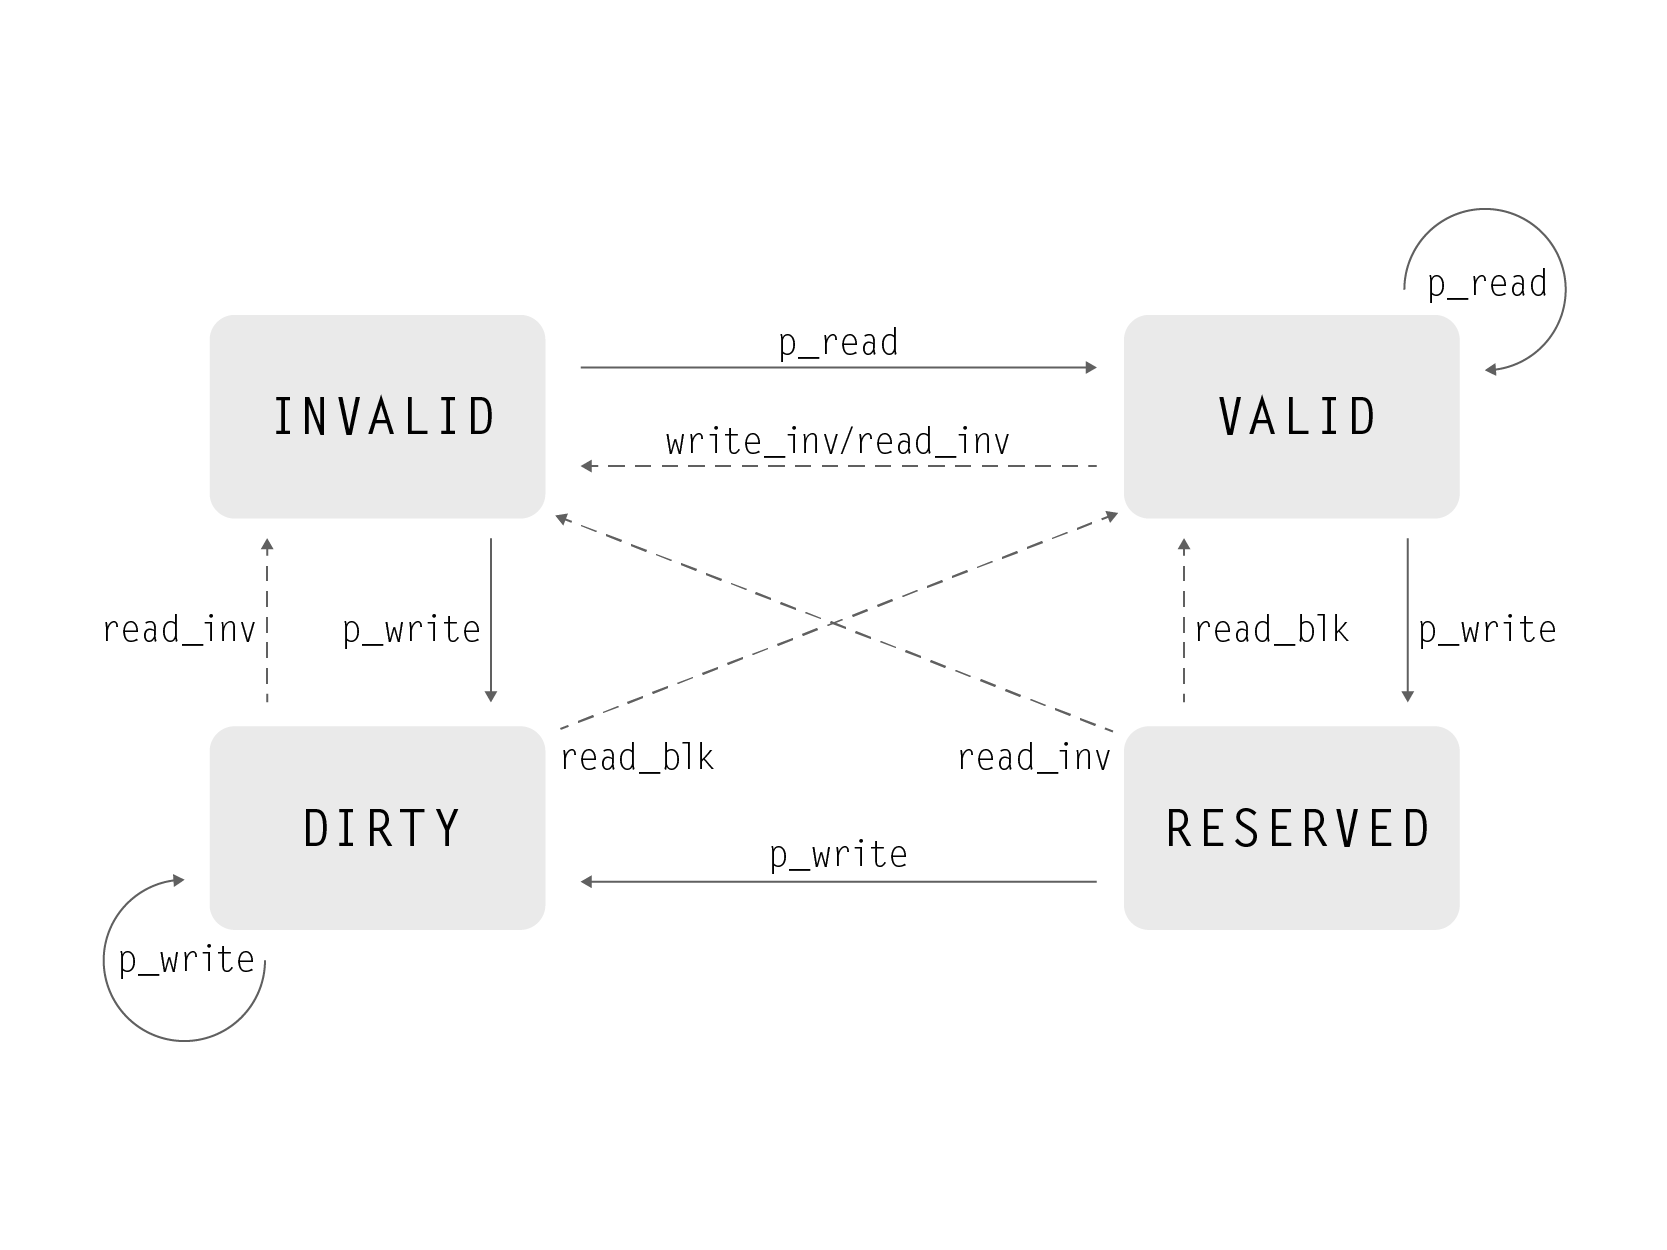
\includegraphics[width=0.9\textwidth]{write-once}
  \label{fig:writeonce-automata}
  \caption{Diagrama de estados do \textit{Write Once}}
\end{figure}






\subsubsection{Firefly}
É um tipo de protocolo \textit{write-update} que foi implementado em estações de trabalho multiprocessada Firefly. A política utilizada entre as caches e a memória é a de \textit{write-through}. Necessita de uma linha especial de barramento para fazer as atualizações, chamado de \textit{shared line}.

\textsc{Transições de Leitura:}
\begin{itemize}
  \item \textbf{Read-Hit:} são feitos sempre na cópia local;

  \item \textbf{Read-Miss:} se existem cópias \textsc{Shared}, as caches fornecem o bloco. Se a cópia está \textsc{Dirty}, a cache fornece o bloco e atualiza a memória. O estado de ambas as cópias muda para \textsc{Shared}. Se não há cópias, a memória fornece uma cópia, que é colocada no estado \textsc{Valid-Exclusive}.
\end{itemize}

\textsc{Transições de Escrita:}
\begin{itemize}
  \item \textbf{Write-hit:} se o bloco estiver \textsc{Dirty} ou \textsc{Valid-Exclusive}, a escrita é local e o novo estado é \textsc{Dirty}. Se a cópia estiver em \textsc{Shared}, todas as cópias e a memória são atualizadas. Se não existe mais compartilhamento, o estado muda para \textsc{Valid-Exclusive};

  \item \textbf{Write-miss:} se a cópia for fornecida pela memória, ela é atualizada localmente e o seu estado fica \textsc{Dirty}. Senão, todas as outras cópias são atualizadas e o novo estado é \textsc{Shared}.
\end{itemize}

\begin{figure}[ht]
  \centering
  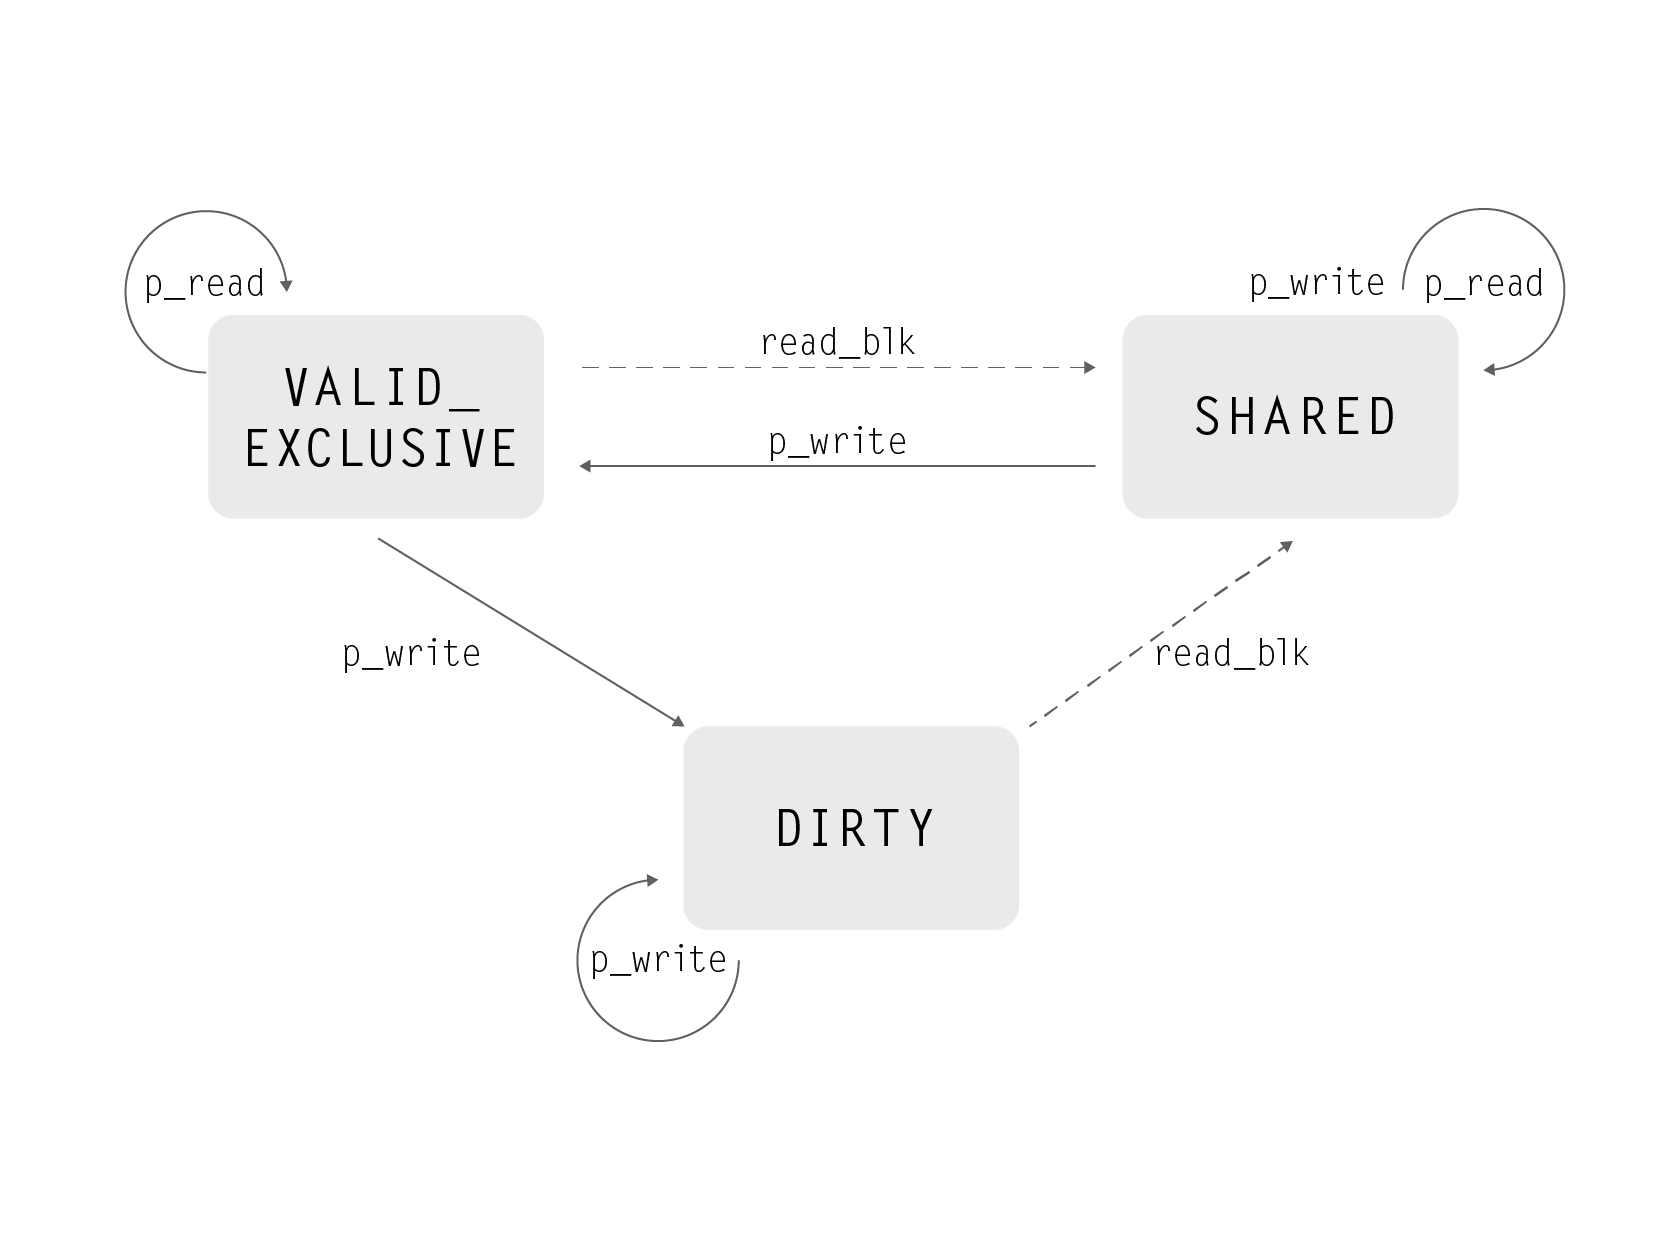
\includegraphics[width=0.9\textwidth]{firefly}
  \label{fig:firefly-automata}
  \caption{Diagrama de estados do Firefly}
\end{figure}


\subsubsection{MSI}
\textsc{Estados}\\
\begin{itemize}
  \item \textbf{Modified} ou Dirty: somente um processador possui uma cópia válida do bloco em sua cache. A cópia da memória principal está incoerente.
  \item \textbf{Shared}: o bloco está presente em diversas caches e está coerente com a memória.
  \item \textbf{Invalid}
\end{itemize}

Este protocol segue a política de cache \textbf{write-back} e é do tipo \textbf{write-invalidate}. \textbf{Note que:}
\begin{itemize}
  \item Ao longo do protocol apenas um processador pode estar no estado \textsc{Modified};

  \item O estado \textsc{Modified} só pode coexistir com estados \textsc{Invalid}.
\end{itemize}

\begin{figure}[ht]
  \centering
  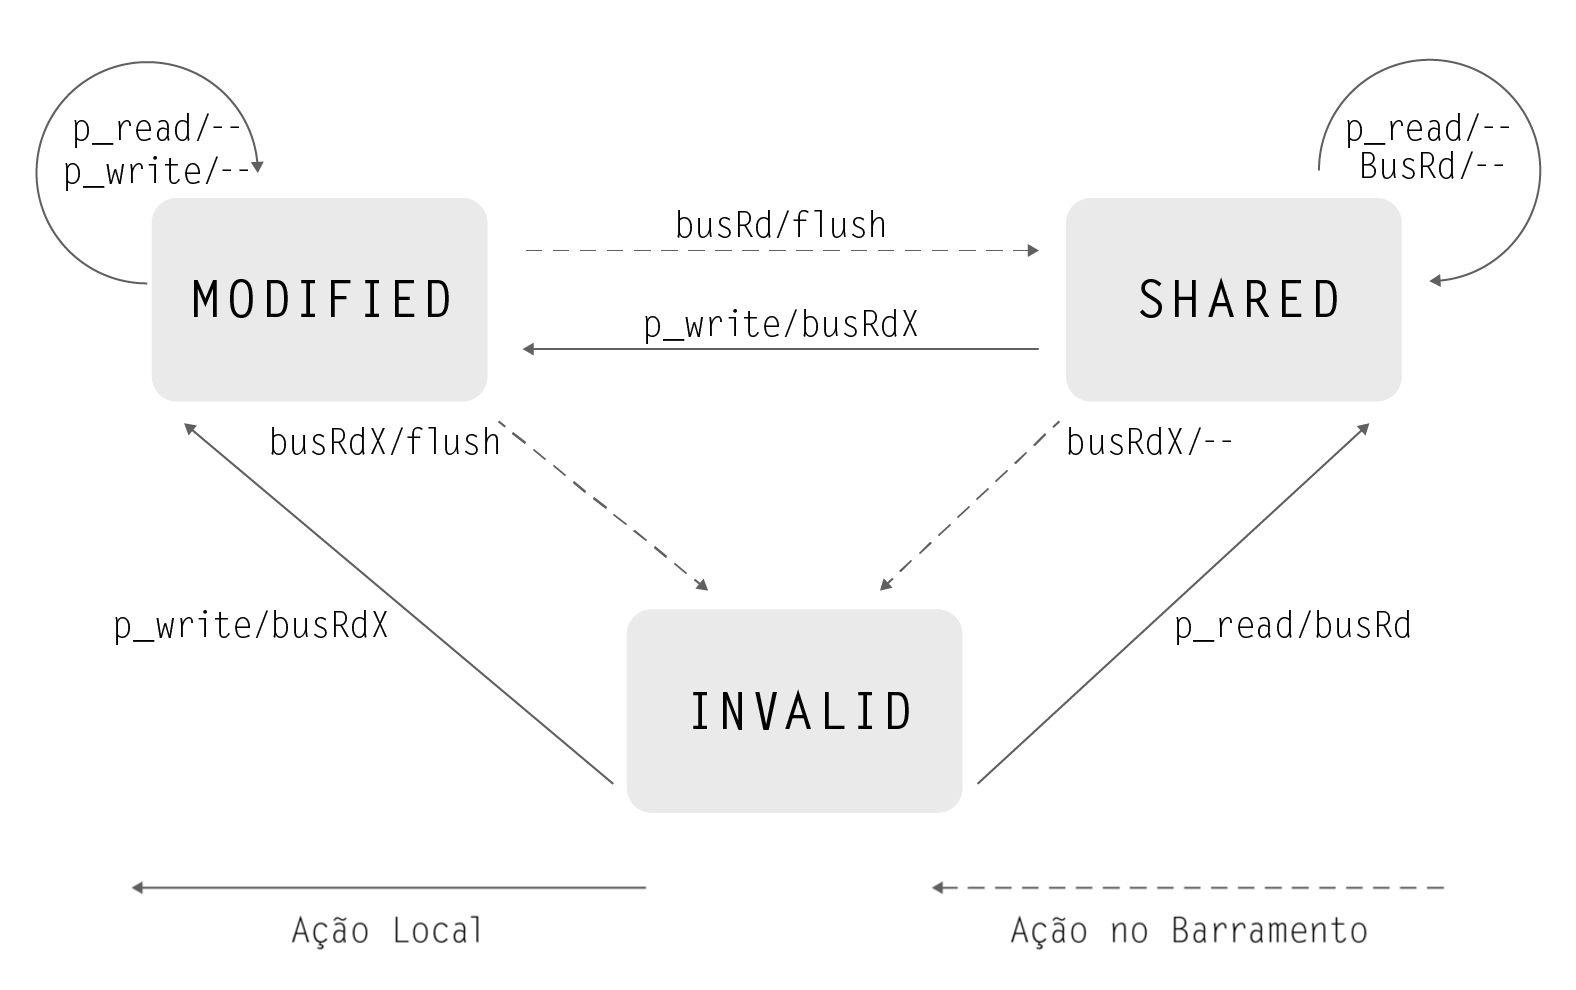
\includegraphics[width=.9\textwidth]{msi}
  \label{fig:msi-automata}
  \caption{Diagrama de estados do MSI}
\end{figure}



\subsubsection{MESI}
Foram propostos para explicitar o estado onde um dado foi lido com a intenção de ser escrito. A inclusão deste terceiro estado diminui o número de transações no barramento para este caso.

Este protocol segue a política de cache \textbf{write-back} e é do tipo \textbf{write-invalidate}.

\begin{figure}[ht]
  \centering
  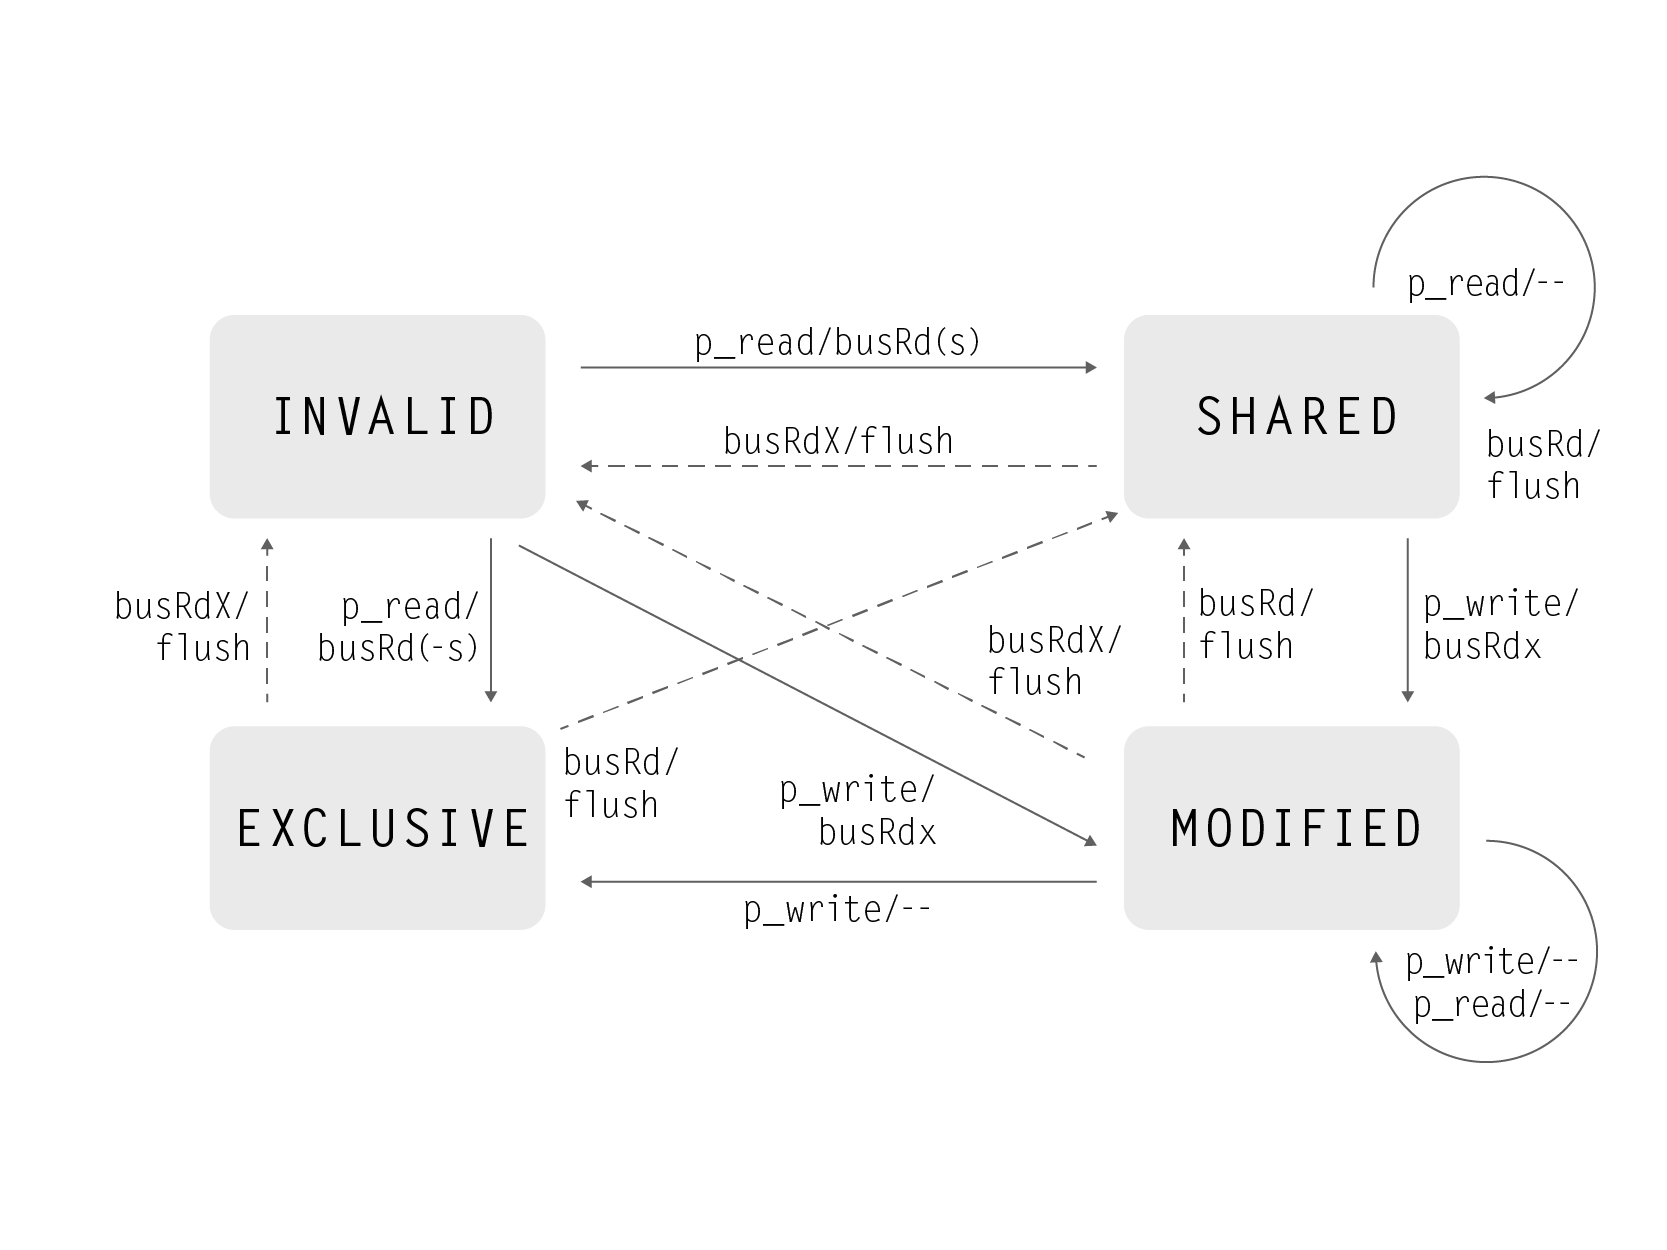
\includegraphics[width=\textwidth]{mesi}
  \label{fig:mesi-automata}
  \caption{Diagrama de estados do MESI}
\end{figure}


\textsc{Observações}\\
Protocolos \textit{write-invalidate} apresentam problemas quando existe um escritor e vários leitores. Para esta situação, podemos reduzir o número de \textit{read misses} se, no primeiro read miss que ocorrer, uma cópia for enviada a todas as caches que possuem o bloco no estado \textsc{Invalid}.

Protocolos \textit{write-update} tem o problema de que algumas atualizações podem ser aplicadas em cópias que não mais serão lidas. Por isso, alguns protocols adicionam estados que representam o número de vezes que um bloco foi alterado sem que nenhuma leitura fosse gerada. Se este número atingir um certo limite, as cópias são invalidadas.




\subsection{Protocolos Baseados em Diretórios}
Em algumas arquiteturas, não dispomos de barramento, logo um \textit{broadcast} tem um custo muito alto. Ao invés de usarmos o snoopy cache, fazemos um multicast somente para as caches que com certeza terão o bloco.

Aqui, a memória possui uma lista dos blocos em cache: para cada bloco nas caches, temos a localização de todos os nodos que possuem uma cópia. Esta lista pode ser centralizada ou distribuída e é chamada de \textbf{diretório}.

Em cada entrada do diretório, ou seja, para cada bloco, temos todas as caches que possuem o bloco e um \textit{dirty bit}, indicando a permissão de escrita.




\subsubsection{Full-map Directories}
Aqui, todas as caches do sistema podem abrigar simultaneamente qualquer bloco de dados. Cada entrada de diretório possui, no mínimo, $N$ bits, onde $N$ representa o número de processadores no sistema. Este bit representa o estado do bloco na cache do processador: se está presente ou ausente. Como exemplo, podemos checar a Figura \ref{fig:cache-fullmap}

\begin{figure}
  \centering
  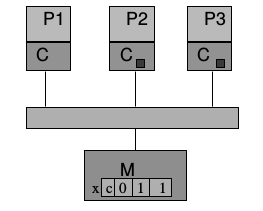
\includegraphics[width=0.6\textwidth]{cache-fullmap}
  \caption{Representação de Diretórios Full-map do estado das caches}
  \label{fig:cache-fullmap}
\end{figure}

\textbf{Escrita}: quando um processador quer escrever, sua cache verifica se o seu bloco local tem permissão de escrita. Caso não, a cache faz \textit{write} para a memória. As demais caches que possuem o bloco recebem o sinal do módulo da memória para invalidar o dado e enviam um \texttt{ACK} para a memória, afim de confirmar. Por fim, o módulo atualiza o diretório e envia a permissão escrita a C3.

Perceba que há um \textit{overhead}: o tamanho de cada entrada de diretório é proporcional ao número de processadores do sistema e isso \textbf{não é escalável}. Por isso, vários esquemas alternativos surgiram.




\subsubsection{Limited Directories}
Propostos com o intuito de \textbf{reduzir o tamanho dos diretórios}. Aqui o número de cópias em cache simultâneas para um bloco particular é limitado.

\begin{definicao}{Dir$_{i}X$}
  Onde $i$ é o número de cópias simultâneas e $X$ pode ser NB (\textit{no broadcast}) ou B (\textit{broadcast}).
\end{definicao}

São similares aos full-map, exceto no caso onde existem mais de $i$ solicitações de leitura simultâneas. Neste caso, podemos tomar duas atitudes:
\begin{itemize}
  \item $\text{Dir}_i\text{NB}$: uma das cópias é invalidada para dar lugar à nova cópia;

  \item $\text{Dir}_i\text{NB}$: caso haja $j$ cópias em leitura e $j > i$, é enviado um \textit{broadcast} na rede para cada operação de coerência.
\end{itemize}

\textbf{Escrita:} quando um processador $P_i$ quer escrever, sua cache $C_i$ verifica se o bloco local em questão está inválido. Caso positivo, solicita uma cópia da memória, a qual pode detectar que já existem cópias em outras caches distintas. A memória escolhe cópia na cache $C_k$ uma para invalidar (se torna \textit{evicted}) e envia o sinal. A cache $C_k$ recebe a invalidação, seta o bloco como inválido e envia uma confirmação \texttt{ACK} para a memória. Por fim, a memória atualiza o diretório, colocando a $C_i$ no lugar de $C_k$ na posição do bloco solicitado e envia a permissão de escrita para $C_i$.




\subsubsection{Diretórios Encadeados}
É um tipo de diretório \textbf{escalável, porém não limita o número de cópias}. A localização das cópias é obtida através de uma cadeia de ponteiros, como mostrado na Figura \ref{fig:cache-chained-dir}.

\begin{figure}[!ht]
  \centering
  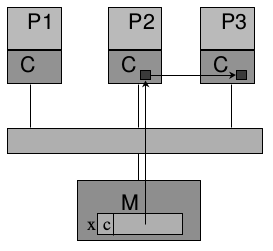
\includegraphics[width=0.6\textwidth]{cache-chained-dir}
  \caption{Representação de Diretórios Encadeados}
  \label{fig:cache-chained-dir}
\end{figure}




\subsubsection{Esquemas Baseados em Software}
Para decidir se o dado é "seguro", temos que marcar todos os dados compartilhados que foram lidos e escritos em algum momento. Marcamos eles como \textit{non-cachable}.

Por fim, precisamos decidir em que fases de um programa uma variável \textit{read-write} pode ser classificada como segura. Ao final da fase, é inserida uma primitiva de invalidação.
